% !TEX root = ../main.tex

\chapter{Bibliographic Study}
\label{ch:bibliographic-study}

\section{Theoretical background}
\label{sec:theory}

\subsection{IEEE-754 single-precision floating point}
Before going into the methods for approximating the sine function, we need to
understand the way real numbers are represented in memory using the IEEE~754
single-precision floating point standard~\cite{ieee754}.

The standard defines arithmetic formats, rounding rules, operations and exception handling~\cite{ieee754}.
For this project specifically we are interested in the specifics of \textbf{binary32}. As its name suggests,
the \textbf{binary32} uses 32 bits to represent a real number:
\begin{figure}[htbp]
  \centering
  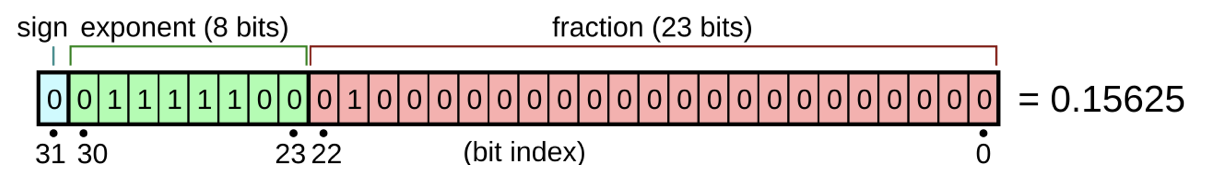
\includegraphics[width=\textwidth]{binary32}
  \caption{The IEEE~754 binary32 (single-precision) format~\cite{wiki_binary32}}
  \label{fig:binary32}
\end{figure}

The most significant bit gives the sign of the number - 0 for positive, 1 for negative values.
Next 8 bits represent the exponent, biased with 127.
The rest of 23 bits represent the mantissa (or fraction) which are the fractional part of
the number with the implicit leading 1 bit for normalized values~\cite{muller2020,wiki_binary32}.
The standard describes special exponents to represent special values like \(\pm 0\), NaN, \(\pm \infty\).

The exponent values $E = 0$ and $E = 255$ are reserved for special values,
as summarized in \cref{tab:special}~\cite{wiki_binary32}.

\begin{table}[htbp]
  \centering
  \caption{Special values in the binary32 format}
  \label{tab:special}
  \begin{tabular}{lll}
    \toprule
    Exponent $E$ & Fraction $f$ & Value \\
    \midrule
    $0$   & $0$      & $\pm 0$ \\
    $0$   & $\neq 0$ & subnormal: $(-1)^{s} \times 2^{-126} \times 0.f$ \\
    $255$ & $0$      & $\pm \infty$ \\
    $255$ & $\neq 0$ & NaN (not a number) \\
    \bottomrule
  \end{tabular}
\end{table}

For a normalized number, with sign bit $b_{31}$, biased exponent $E$ stored as an
8-bit unsigned integer and a 23-bit fraction, the represented value is
\begin{equation}
  (-1)^{b_{31}} \times 2^{(b_{30} b_{29} \dots b_{23})_2 - 127}
  \times (1.b_{22} b_{21} \dots b_{0})_2
  \label{eq:binary32-bits}
\end{equation}
which can also be written as a sum over the fraction bits~\cite{muller2020,wiki_binary32}:
\begin{equation}
  \text{value} = (-1)^{\text{sign}} \times 2^{(E-127)} \times
  \left( 1 + \sum_{i=1}^{23} b_{23-i}\, 2^{-i} \right)
  \label{eq:binary32}
\end{equation}


\subsection{Elementary function evaluation}
Following~\cite{muller2020}, the term \emph{elementary functions} refers to
the most widely used mathematical functions: $\sin$, $\cos$, $\tan$, $\sin^{-1}$,
$\cos^{-1}$, $\tan^{-1}$, $\sinh$, $\cosh$, $\tanh$, $\sinh^{-1}$, $\cosh^{-1}$,
$\tanh^{-1}$, as well as exponentials and logarithms in bases $2$, $e$ and $10$.
These elementary functions can only be approximated, they cannot be computed exactly
with a finite number of operations, as mentioned in \cref{sec:motivation}.

\paragraph{Measuring accuracy.}
Since an elementary function can only be approximated, the quality of an
implementation is described7 by the error between the computed result
$y^{*}$ and the exact result $y = f(x)$. Two measures are commonly used: the
\emph{absolute error}, $|y^{*} - y|$, and the \emph{relative error},
$|y^{*} - y| / |y|$. The ideal behaviour is \emph{correct
rounding}, in which the implementation always returns the floating-point number
nearest to the exact result~\cite{muller2020}.


\subsection{AXI-4 Streaming interface}
In a dataflow architecture, processing is organized as a pipeline of independent
modules, where each module receives data from the previous one and passes its
results to the next. Since modules may need a different number of clock cycles to
process a data item, they rarely run at the same rate: a fast sender feeding a
slower receiver must stall until the receiver can accept new data, so the
throughput of the whole pipeline is bottlenecked by its slowest stage. Moreover, if a
sender kept transmitting while its receiver was busy, data would be lost. A flow
control mechanism is therefore needed between the stages~\cite{scs_lab04}.

The AXI4-Stream protocol is a great interface to connect modules that need to exchange
data. It connects a sender and a reciever together relying on a \textbf{ready/valid}
handshake principle.

The interface consists of 5 main signals: a shared \textbf{CLOCK}, a global \textbf{RESET} (active LOW),
the \textbf{DATA} lines, and 2 "control" bits: \textbf{VALID} (from the sender to the reciever)
and \textbf{READY} (from the reciever to the sender)~\cite{scs_lab04}. Of course, the interface provides
other optional signals, but the ones mentioned above are mandatory for reliable transfer of data between the modules.

Linking two modules together is simply done by connecting the output of the "sender" module to the inputs of the
"reciever" module.
\begin{figure}[htbp]
  \centering
  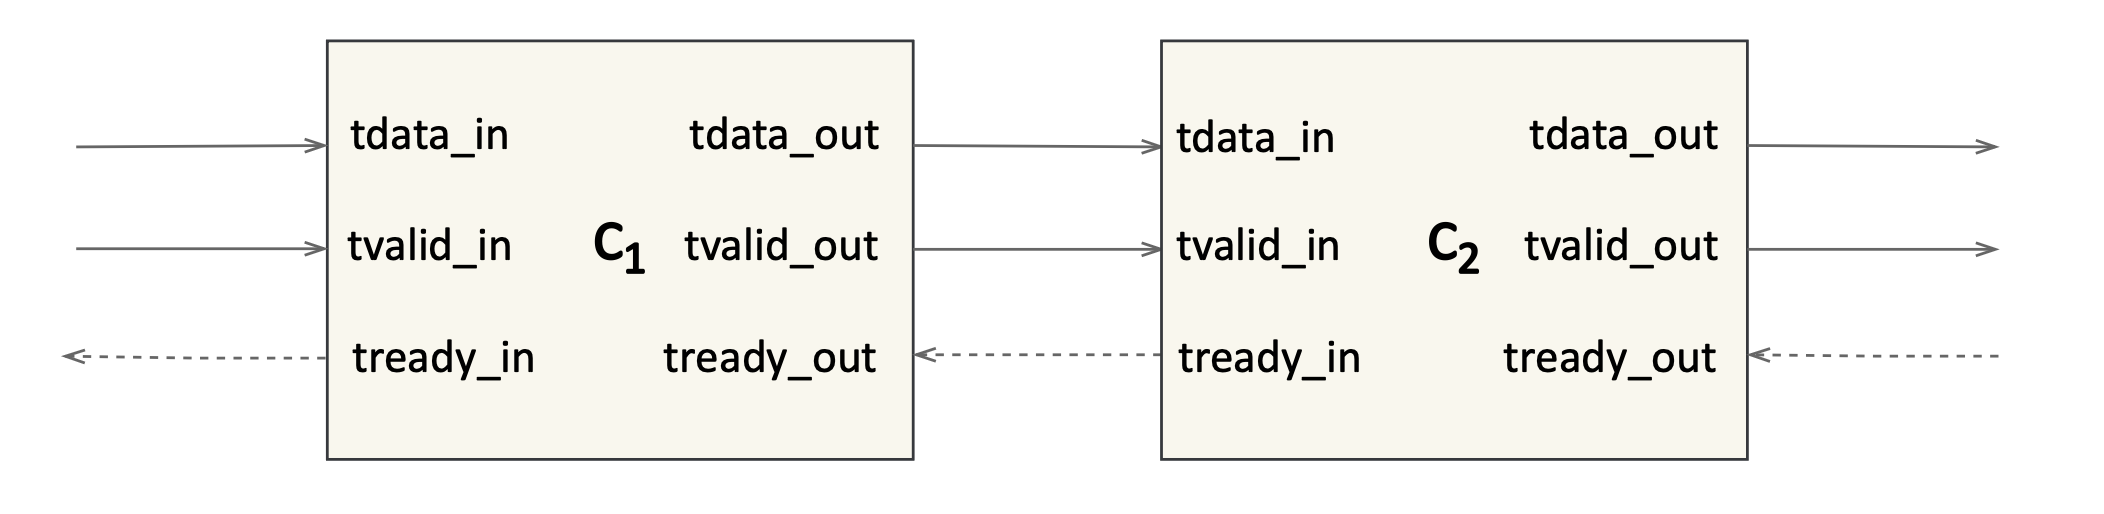
\includegraphics[width=\textwidth]{axi4-2modules.png}
  \caption{Two interconnected components using AXI4-Stream Interface~\cite{scs_lab04}}
  \label{fig:axi4-2modules}
\end{figure}

\paragraph{The core HANDSHAKE rules.}
As mentioned above, the \textbf{TVALID} and \textbf{TREADY} signals dictate when the information is transmitted
across. This two-way mechanism allows both the sender and the reciever to control when the information is passed.
The AXI4-Stream protocol imposes a very important rule, that is, for a data transfer to happen, both \textbf{TVALID}
and \textbf{TREADY} signals must be asserted during the same clock cycle~\cite{scs_lab04}.
Am ramas la handshake.


\section{Existing approaches for approximations}
\label{sec:existing}

\subsection{Table-based methods}

\subsection{Shift-and-add algorithms (CORDIC)}
pe foaie deocamdata

\subsection{Polynomial approximation}

\subsection{Bit-manipulation techniques}

\subsection{Vendor IP cores}

\section{Work plan}
\label{sec:workplan}

\begin{table}[htbp]
  \centering
  \caption{Targets for each project meeting}
  \label{tab:workplan}
  \begin{tabularx}{\textwidth}{lX}
    \toprule
    Meeting & Target \\
    \midrule
    PM 1 & Pick the project and begin studying\\
    PM 2 & Introduction and bibliographic study\\ 
    PM 3 & Initial design for the two approximation methods\\
    PM 4 & Updated design of the two approximation methods\\
    PM 5 & Start implementing methods in hardware\\
    PM 6 & Continue implementing in hardware and start testing\\
    PM 7 & Finish testing and present final project\\
    \bottomrule
  \end{tabularx}
\end{table}
